\documentclass{article}

\usepackage[noend]{algpseudocode}
\usepackage[margin=1in]{geometry}
\usepackage{enumitem}
\setlist{wide,labelwidth=!,labelindent=0pt,topsep=0pt}
\usepackage{cprotect}
\usepackage{listings}
\usepackage{tikz-qtree}
\usepackage{graphicx}
\usepackage{float}
\tikzset{every tree node/.style={minimum width=.1in,draw,circle},
         blank/.style={draw=none},
         edge from parent/.style=
         {draw,edge from parent path={(\tikzparentnode) -- (\tikzchildnode)}},
         level distance=5mm}

\setlength{\headsep}{0.5 in}
\setlength{\parindent}{0 in}
\setlength{\parskip}{0.1 in}
\addtolength\topmargin{-1cm}
\textheight  9.4in

\usepackage{amsmath,amsfonts,graphicx,multicol, color}
\usepackage[normalem]{ulem}

\newcommand{\todo}{\textcolor{red}}
\newcommand{\red}{\textcolor{red}}
\newcommand{\algorithm}{\textbf{Algorithm:} }
\newcommand{\proof}{\textbf{Proof:} }
\newcommand{\intuition}{\textbf{Intuition:} }
\newcommand{\complexity}{\textbf{Complexity:} }

\usepackage{url}

%\def\IsSolution{1}   % Uncomment to debug solutions. Note: Makefile generates both discussion and solution automatically.

%
% Define two macros
%   \soln{}     --- contents appear only in solution
%   \notsoln{}  --- contents appear only if not solution

\usepackage{etoolbox}
\ifx\IsSolution\undefined
 \newcommand{\notsoln}[1]{#1}
 \newcommand{\soln}[1]{}
 \newcommand{\thesoln}[1]{}
\else
  \newcommand{\notsoln}[1]{}
  \newcommand{\soln}[1]{#1}
  \newcommand{\thesoln}[1]{{\color{red}\textbf{Solution:} #1}}
\fi


%
% The following macro is used to generate the header.
%
\newcommand{\header}[1]{
   \pagestyle{myheadings}
   \thispagestyle{plain}
   \newpage
   \setcounter{page}{1}
   \noindent
   \begin{center}
   \framebox{
      \vbox{\vspace{2mm}
    \hbox to 6.28in { {\bf COMPSCI 311: Introduction to Algorithms
		\hfill Spring 2020} }
       \vspace{4mm}
       \hbox to 6.28in { {\Large \hfill Homework #1 \soln{Solutions} \hfill } }
       \vspace{2mm}
       \hbox to 6.28in { Released 4/2/2020 \hfill Due 4/15/2020 11:59pm in Gradescope}
      \vspace{2mm}}
   }
   \end{center}
   \markboth{Homework #1}{Homework #1}

%   \vspace*{4mm}
}

\newcounter{problem}
\newcommand{\prob}{\addtocounter{problem}{1}\noindent {\bf Problem \theproblem.} ~}

\begin{document}
\header{5}

\textbf{Instructions.} You may work in groups, but you must write solutions yourself.
List collaborators on your submission.   Also list any sources of help (including online
sources) other than the textbook and course staff.

If you are asked to design an algorithm, please provide: (a) the pseudocode or precise description in words of the algorithm, (b) an explanation of the intuition for the algorithm, (c) a proof of correctness, (d) the running time of your algorithm and (e) justification for your running time analysis. 

%\medskip

\textbf{Submissions.} Please submit a PDF file. You may submit a scanned handwritten document, but a typed submission is preferred. Please assign pages to questions in Gradescope.

%\medskip

%\fbox{\textbf{Efficiency}. The algorithms you design should be polynomial-time, unless something else is stated.}
  
\begin{enumerate}[topsep=0pt]

\item (10 points) \textbf{Increasing Capacities} 

The claim is incorrect. Consider a graph
\begin{figure}[H]
  \centering
  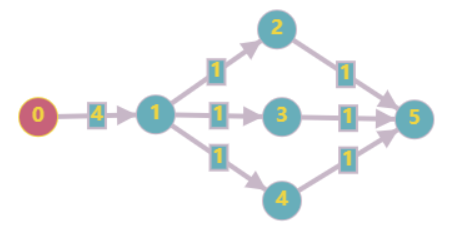
\includegraphics[width=5cm]{Q1.png}
\end{figure}

in which the flows goes from $0$ to $5$. Currently, the minimum cut capacity is 3 which is $(\{0,1\},\{2,3,4,5\})$.
However, when add 1 to the capacity of every edge in the network,
the minimum cut capacity would be 5 which is $(\{0\},\{1,2,3,4,5\})$, 
and the capacity of the cut $(\{0,1\},\{2,3,4,5\})$ becomes 6 which is not the minimum cut.
This operation changes the minimum cut in the network.



\item (10 points) \textbf{Greedy Flow} 

Consider the graph

\begin{figure}[H]
  \centering
  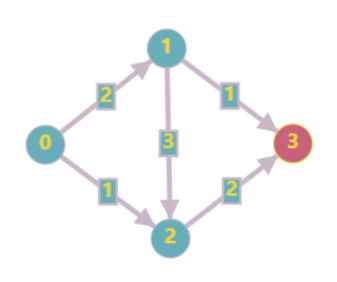
\includegraphics[width=3cm]{Q2.1.png}
\end{figure}

in which the flows goes from $0$ to $3$.
Initialize all flows as 0.

Consider augmenting path $0,1,2,3$, after the first step, we have

\begin{figure}[H]
  \centering
  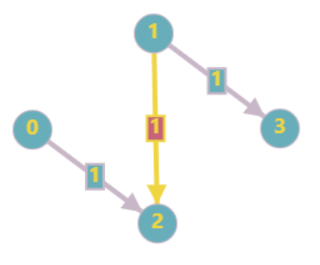
\includegraphics[width=3cm]{Q2.2.png}
\end{figure}

and there is no more augmenting path in this graph, so done.

After the algorithm, we have a flow with size 2 from $0$ to $3$, 
however, clearly the maximum flow should be 3.

So, this algorithm does not compute a maximum flow.

\item (20 points) \textbf{Cold War Flow}

\algorithm
Consider every path has capacity 1.

Use Capacity-scaling Algorithm to get the max flow F and keep the final residual graph $G'$.

In $G'$, from $s$, do a DFS search to find all nodes reachable from $s$ as $A$, $B=E\setminus A$.

From all edges in $G$, find all edges $E'$ that goes from $A$ to $B$ (forward edges).

The max flow is the sum of the capacities of $E'$, and the set of $k$ edges should be
some arbitrary edges in the set $E'$. If $|E'|<k$, then it should contain all edges in $E'$
and any other edges with count $k-|E'|$.

\intuition
Simply get the min-cut in the graph and cut $k$ edges from the min-cut forward edges,
because the min-cut in the max-flow must be fulfilled, and remove edges from there must reduce the flow through the min-cut,
so it will reduce the max-flow by the capacities removed from there.

\proof
Consider $f$ be the maximum flow in $G$, because all capacities are 1, 
we cannot get flow less than $f-k$ by removing $k$ edges form $G$.

According to the max-flow min-cut theorem, there is an min $s-t$ cut with $f$ forward edges in $G$,
in which all these edges are in full capacity. 
Removing any number of edges from this cut, the min-cut of the new graph would not change,
because the capacities of the forward edges in any other $s-t$ cuts would only reduce by the value no larger than the number of removed edges.
By removing $k$ edges from min $s-t$ cut, we will get $f-k$ new maximum flow, which is the smallest possible max-flow.
So, removing $k$ edges from the min $s-t$ cut would definitely reduce the maximum flow in $G$ as much as possible.

We know that if we have found the max-flow network,
the $s-t=(A,B)$ cut is a min-cut iff all the capacities of the are fulfilled from $A$ to $B$,
so all the paths $s\rightarrow t$ in the residual stops at the min-cut.
Therefore, the connected component contains $s$ in the residual graph is $A$ in the min-cut.

\complexity
The complexity of Capacity-scaling is $O(m^2)$, because $1+\lfloor C_{max}\rfloor=1+0=1$
The complexity of DFS is $O(m+n)$. Because we are searching a connected component, we have $n\le m+1$, so the complexity is $O(m+m+1)=O(m)$
The complexity of find all edges in $E'$ and extract $k$ edges is $O(m)$.

So, the total complexity is $O(m^2+m+m)=O(m^2)$

\item (20 points) \textbf{Acyclic Flows} 

(a) \algorithm
Use Ford-Fulkerson to find the max-flow graph $F=(V,E)$.
Use DFS to find a cycle in $F$ 
(if there is a back-edge, extract all edges from the node the back-edge goes to to the current node).
The DFS ends when all edges are visited or there is a back-edge (infers cycle).
Reduce the weight in the cycle by the minimum edge weight in the cycle.
Iteratively do this until there is no cycle, and the new graph is the acyclic max-flow graph.

\intuition
Find cycles in the original max-flow graph and reduce all edges in the cycle by the smallest weight in the cycle,
therefore the cycles can be cancelled iteratively.

\proof
To prove this algorithm is correct, just need to prove that cancel a cycle would not affect the max flow in the graph.
We know that in a max-flow graph, any $s-t$ cut would have the same flow value for $f_{in}-f_{out}$ 
(out means edges go out of $s$ set, and in means edges go into $s$ set).
For augmenting edges in the cycle (it is a simple cycle which contains only one cycle as described in the algorithm), 
it only affects cuts that cut through the cycle (one set only contains part of the vertices in the cycle).
Therefore, there must be exactly one edge in $e_{in}$ and one edge out $e_{out}$ which are in the cycle.
So, the net flow $f$ in this cut is $f+w-w=f$ when reduce weight $w$ for $e_{in}$ and $e_{out}$,
in conclusion, the overall flow is not affected by the augmenting for the cycle.

Because we keep augmenting until there is no cycle, and each augmenting keeps the max-flow,
the final graph must be a acyclic max-flow graph.

\complexity
F-F algorithm is $O(mnC_{max})$, find cycle and augmenting flow takes $O(n)$ for each iteration,
and there are at most $O(m)$ iterations because at most $m$ edges can be cancelled,
so in total $O(mn)$ for the transformation part.

Therefore, the total complexity is $O(mnC_{max}+mn)=O(mnC_{max})$

(b)\algorithm
Find the max-flow network $F=(V,E)$ from $G$ and its residual graph $R=(V,E_R)$ using Ford-Fulkerson.
Check if there is a cycle in $F$ using DFS (starts from $s$ as described in (a)). If there is any cycle,
then not every maximum flow in $G$ is acyclic, because we already found a cyclic one.

If $F$ is acyclic, for $H=(V,E_R\setminus E)$, check if there is a cycle in $H$ using DFS.
The DFS should start from any node, and ends if all nodes have been visited, or there is a back-edge.
If there is a cycle in $H$, then not every maximum flow in $G$ is acyclic.

\intuition
Get the free capacities (the capacities that are not used in the max-flow network for the original graph) of a acyclic max-flow graph 
(if its not acyclic, then there must be at least one cyclic max-flow network),
and check if these remained capacities can form a cycle.

\proof
The first part of the algorithm is simple, because it just directly checks if the current max-flow network is acyclic.

In the second part, we can see that $H$ contains all the backward edges in $R$. If a cycle is found in $H$,
add some weight $k$ to all corresponding edges in $F$ 
(for example, if $(u,v)$ in a cycle in $H$, we can add weight $k$ to $(u,v)$ in $F$, or create an edge $(u,v)$ in $F$ with weight $k$).
The new graph must be cyclic because the new edges added to $F$ will form a cycle as they are just the cycle found in $H$ 
and the max-flow remains the same as proved in (a).

For any set of edges that are not in a simple cycle, plus their weights by a constant $k>0$ must affect the flow of some $s-t$ cut,
because we can simply find some $s-t$ cut that cross exactly one of the edges in the set, 
and the flow cross the cut would be $f-k$ or $f+k$ where $f$ is the max flow value. 
Also, because the edges are the remained capacities of the original graph, 
they are the only weights that can be added to $F$ to satisfies the capacity limit.

Therefore, this algorithm can find a cyclic max-flow network if there exists one.

\complexity
F-F algorithm is $O(mnC_{max})$, the first DFS is $O(mn)$ same as in (a). 
To get $H$, we need $O(m)$, because it just take out part of the edges from $R$ which has at maximum $2m$ edges.
The second DFS is still $O(mn)$, because it is just the same as the first DFS but in a different graph which has same vertices 
and the edges will not exceeds $O(m)$.
So, the total complexity is $O(mnC_{max}+mn+m+mn)=O(mnC_{max})$

\item \textbf{(20 points) Separating Edges} 

(a) Consider a path $P=s\rightarrow t$ which does not have edge in $\delta S$.
We know that $s\in S,t\in T$, and an edge is in $\delta S$ iff it starts from some nodes in $S$ and ends at some nodes in $T$, 
because $(S,T)$ is a $s-t$ cut which determines all nodes not in $S$ must be in $T$.
Therefore, if $P$ does not have edge in $\delta S$, it cannot have any edge in $T$, means it cannot reach $t$.
As a result, any arbitrary path $P(s\rightarrow t)$ must have at least one edge in $\delta S$, so $\delta S$ separates $s$ and $t$.

(b) Clearly, a non $s-t$ cut has no relationship with separating $s,t$. 
For non $s-t$ cut $(A,B)$, $\delta A$ cannot separate $s,t$, because $s-t$ must be in the same set.

Consider that the edges in $X$ does not contain any $\delta S$.
So, for all $s-t$ cut $(S,T)$, $\delta S\not\subseteq X$.

As proved in (a), we know that an edge is in $\delta S$ iff it starts from some nodes in $S$ and ends at some nodes in $T$ for the $s-t$ cut $(S,T)$.
That means, for any $\delta S$, there is a cut $(S,T)$, and that $\delta S$ separates $s$ and $t$.

When removing any edge from $\delta S$ to form $\delta S'$, there is a edge from $S$ to $T$ not in $\delta S'$, a path can go through $S$ to $T$, 
so $\delta S'$ does not separate $s,t$, therefore $\delta S$ is the minimum set of edges that separates $s,t$ for cut $(S,T)$.

Therefore, $\forall\delta S\not\subseteq X$, $X$ does not separate $s,t$, 
contradictory to the premise that $X$ separates $s$ and $t$,
gives that $\exists\delta S \subseteq X$ for $s-t$ cut $(S,T)$

(c) As proved in (b), we know that for each $s-t$ cut $(S,T)$, $\delta S$ is the minimum edges that separates $s,t$.
Also, for $Y$ be any subset of edges that separates $s,t$, we know that $\delta S \subseteq Y$.
Therefore, for some subset of edges that separates $s,t$, it must be at least some $\delta S$,
so the minimal $X$ must be some $\delta S$.

Because $\delta S$ is determined by $s-t$ cut $(S,T)$, so there must also be a cut for $\delta S$.
 
\item \textbf{(20 points) Incremental Change} 

(a) \algorithm

Construct $G'$ from $G=(V,E),f^*=(V,E^*)$

Do BFS from $s$ to $t$ to find the simple path $P(s\rightarrow t)$
in $G'$ in which $w(e'(u,v))$ has increased by 1.

If there is such a path, the flow of each edge in the path is increased by $1$.
Else, the change of capacity does nothing.

\intuition
Just try to find an augmenting path.

\proof
When $c(e)>w(e^*)$, $e$ is not in the min-cut of $G$, so increase its capacity has no effect.

Consider $c(e)=w(e^*)$, the updated graph is $G_u$, and its residual graph is $G_{u_f}$.
Because we only increase the capacity by 1 for a single edge,
the max-flow $f_u$ of $G_u$ must $m(f_u)\le m(f^*)+1$.
If the flow can be augmented, 
there must be a path $P(s\rightarrow u\rightarrow v\rightarrow t)$,
and the bottleneck of $P$ must be $1$,
because that is the only edge we changed.
Therefore, $m(f_u)=m(f^*)+1$ in this case, which is the maximum flow possible.
If the flow cannot be augmented, the flow is at maximum as proved in the F-F algorithm because this flow is a flow of $G_u$.

So, the algorithm gives the correct answer.

\complexity
$O(m+n)$. 
To construct $G'$, $O(m)$ is required, 
as it just iterates through all the edges. 
$O(m+n)$ for the BFS, $O(m)$ for augmenting.

(b) \algorithm
If $c(e)>w(e^*)$, do nothing.
Else, construct $G_f$ from $G=(V,E),f^*=(V,E^*)$,
do 2 BFS to find simple path $P(t\rightarrow v),Q(u\rightarrow s)$ in $G_f$
for which all the edges have flow greater than 0.
Consider $R=P|(v,u)|Q$ in $G_f$, push back the flow in $R$ by 1 to the forward edges, 
then reduce the weight of the forward edge $(u,v)$ by 1.
The new residual graph is $G_f'=(V,E_f')$.

Perform a BFS search on $G_f'$ from $s\rightarrow t$ to find an augmenting path.
If there is such a path, augment it and update $G_f'$.

Convert the residual graph $G_f'$ to a flow network by delete all forward edges
and inverse the directions of the backward edges to get the final flow network.

\intuition
Just reduce $1$ from a flow path that passes $e(u,v)$,
and then augment the new flow network by once.

\proof
When $c(e)>w(e^*)$, $e$ is not in the min-cut of $G$, so decrease its capacity won't change the flow.

So, only consider $c(e)=w(e^*)$. The updated graph is $G_u$.
We can say that for the max-flow $f_u$ in $G_u$, $m(f^*)-1\le m(f_u)\le m(f^*)$.
By doing the push back, we get $m(f_u')=m(f^*)-1$, which is the smallest possible flow.
The $f_u'$ might not be optimal.

By trying augmenting $f_u'$, the $m(f_u')$ can increase maximum by $1$,
because decrease the capacity cannot increase the min-cut, 
therefore the max possible min-cut is still $m(f^*)$.
Because the smallest unit is 1 in integer, this increment can be done in one augment.
Therefore, this one augment can update the flow to max-flow.
Also, as proved in (a), if no augment path, the flow is already at maximum.

Therefore, the algorithm is correct.

\complexity
$O(m+n)$.
The two BFS are $O(m+n)$, combing the two paths and push back the flow is $O(m)$.
Then, the BFS takes $O(m+n)$, and the deletion and inversion takes $O(m)$ as it can be done by a loop in the edge set.
So, the final complexity is $O(m+n+m+n+m+n+m+m)=O(m+n)$


\item \textbf{(0 points).} How long did it take you to complete this assignment?

\end{enumerate}


\end{document}
